\documentclass[11pt, a4paper]{article}

\usepackage[utf8]{inputenc}
\usepackage[english, spanish]{babel}
\usepackage[left=25mm, right=25mm, top=35mm, bottom=30mm, headheight=35mm]{geometry}
\usepackage{graphicx}
\usepackage{float}
\usepackage{xcolor}
\usepackage{fancyhdr}
\usepackage{hyperref}
\usepackage{setspace}
\usepackage{indentfirst}

\usepackage{ucs}
\DeclareUnicodeCharacter{2500}{\textSFii}

% Syntax customization with minted package
\usepackage{minted}
\usemintedstyle{nord-darker}
\usemintedstyle[zsh]{gruvbox-light}
\setminted{
  breaklines,
  linenos,
  frame=lines,
  fontsize=\normalsize
}
\newcommand{\mj}[1]{\mintinline[style=gruvbox-light]{java}{#1}}

% Define background color
\definecolor{background}{HTML}{2E3440}

% Variables
\newcommand{\university}{Universidad Nacional de San Agustín de Arequipa}
\newcommand{\faculty}{Facultad de Ingeniería de Producción y Servicios}
\newcommand{\program}{Escuela Profesional de Ingeniería de Sistemas}
\newcommand{\semester}{2024 - A}
\newcommand{\course}{img/data_structures.png}
\newcommand{\topic}{img/trie_tree.png}
\newcommand{\professor}{Edson Luque Mamani}
\newcommand{\students}{Jorge Luis Mamani Huarsaya\\Victor Narciso Mamani Anahua}
\newcommand{\mydate}{27 de junio, 2024}

% Just parts and chapters numbered
\setcounter{secnumdepth}{0}

% Head and foot customization
\pagestyle{fancy}
\lhead{\raisebox{-0.2\height}{
\includegraphics[width=4cm]{img/logo_unsa.png}}}
\chead{\fontsize{8}{8}\selectfont \university \\ \faculty \\ \textbf{\program}}
\rhead{\raisebox{-0.2\height}{
\includegraphics[width=3.5cm]{img/logo_episunsa.png}}}
\lfoot{Semestre \semester}
\cfoot{}
\rfoot{Pág. \thepage}

\begin{document}

\begin{titlepage}
	\centering
	\includegraphics[width=15cm]{\course} \par
  \vfill \vfill
	\includegraphics[width=15cm]{\topic}\par
  \vfill \vfill
  {\textbf{Profesor(a):} \par}
	\professor \vfill
  {\textbf{Estudiantes:} \par}
	\students \vfill
	{\large \mydate \par}
\end{titlepage}

\section{Implementación de un Trie Tree en Java}
Un Trie es una estructura de datos especializada que se utiliza para almacenar un conjunto de cadenas, generalmente para realizar búsquedas rápidas de palabras. Se detallará el funcionamiento de cada método y la importancia de los campos establecidos en la clase.

\section{Estructura de la Clase}
A continuación se presenta la implementación de la clase \texttt{Trie}:

\begin{minted}[bgcolor=background]{java}
import java.util.HashMap;
import java.util.Map;

public class Trie implements ITrie {
  private TrieNode root;

  public Trie() {
    // El nodo raiz que representa el caracter nulo
    root = new TrieNode('\0');
  }

  private static class TrieNode {
    int count = 0;
    char ch;
    Map<Character, TrieNode> children;
    boolean isEndOfWord;

    public TrieNode(char ch) {
      children = new HashMap<>();
      isEndOfWord = false;
      this.ch = ch;
    }
  }
\end{minted}

\subsection{Campos de la Clase}
\begin{itemize}
  \item \texttt{root}: Es la raíz del Trie, un nodo especial que no representa ningún carácter (\texttt{'\textbackslash0'}).
  \item \texttt{TrieNode}: Clase estática interna que representa un nodo en el Trie.
  \begin{itemize}
    \item \texttt{count}: Cuenta las veces que una palabra termina en este nodo.
    \item \texttt{ch}: Caracter que representa el nodo.
    \item \texttt{children}: Mapa de hijos, donde la clave es un carácter y el valor es otro nodo \texttt{TrieNode}.
    \item \texttt{isEndOfWord}: Indica si este nodo es el final de una palabra.
  \end{itemize}
\end{itemize}

\section{Métodos de la Clase}
La clase \texttt{Trie} implementa los métodos definidos en la interfaz \texttt{ITrie}. A continuación se detallan cada uno de estos métodos.

\subsection{Inserción de Palabras}
\begin{minted}[bgcolor=background]{java}
@Override
public void insert(String word) {
  TrieNode current = root;
  for (char ch : word.toCharArray())
    current = current.children.computeIfAbsent(ch, c -> new TrieNode(c));

  current.isEndOfWord = true;
  current.count++;
}
\end{minted}

Este método inserta una palabra en el Trie. Recorre cada carácter de la palabra y lo inserta en el Trie si no está presente. Utiliza el método \texttt{computeIfAbsent} de \texttt{HashMap} para agregar un nuevo nodo si el carácter no existe en los hijos actuales. Al final de la palabra, marca el nodo como el final de una palabra (\texttt{isEndOfWord}) y aumenta el contador (\texttt{count}).

\subsection{Búsqueda de Palabras}
\begin{minted}[bgcolor=background]{java}
@Override
public boolean contains(String word) {
  TrieNode current = root;
  for (char ch : word.toCharArray()) {
    current = current.children.get(ch);
    if (current == null)
      return false;
  }
  return current.isEndOfWord;
}
\end{minted}

Este método verifica si una palabra está contenida en el Trie. Recorre cada carácter de la palabra y verifica si existe en el Trie utilizando el método \texttt{get} de \texttt{HashMap}. Si al final de la palabra, el nodo actual es el final de una palabra, retorna \texttt{true}, de lo contrario, \texttt{false}.

\subsection{Obtención de Palabras}
\begin{minted}[bgcolor=background]{java}
@Override
public String get(String word) {
  TrieNode current = root;
  for (char ch : word.toCharArray()) {
    current = current.children.get(ch);
    if (current == null)
      return null;
  }
  return current.isEndOfWord ? word : null;
}
\end{minted}

Este método retorna la palabra si está contenida en el Trie. Sigue la misma lógica que el método \texttt{contains}, pero retorna la palabra en lugar de un valor booleano.

\subsection{Eliminación de Palabras}
\begin{minted}[bgcolor=background]{java}
@Override
public boolean remove(String word) {
  return delete(root, word, 0);
}

private boolean delete(TrieNode current, String word, int index) {
  if (index == word.length()) {
    if (!current.isEndOfWord)
      return false;

    current.isEndOfWord = false;
    return current.children.isEmpty();
  }

  char ch = word.charAt(index);
  TrieNode node = current.children.get(ch);
  if (node == null)
    return false;

  boolean shouldDeleteCurrentNode = delete(node, word, index + 1);
  if (shouldDeleteCurrentNode) {
    current.children.remove(ch);
    return current.children.isEmpty();
  }
  return false;
}
\end{minted}

El método \texttt{remove} elimina una palabra del Trie. Utiliza un método recursivo \texttt{delete} que elimina los nodos si ya no son necesarios. 

\subsubsection{El Método \texttt{delete}}
El método \texttt{delete} es el núcleo del proceso de eliminación. A continuación se explica paso a paso su funcionamiento:

\begin{itemize}
  \item \textbf{Caso Base:} Si el índice ha alcanzado la longitud de la palabra (\texttt{index == word.length()}), se verifica si el nodo actual marca el final de una palabra (\texttt{current.isEndOfWord}). Si no es así, significa que la palabra no está en el Trie y se retorna \texttt{false}. Si lo es, se desmarca como el final de una palabra y se retorna \texttt{true} si el nodo no tiene hijos, indicando que este nodo puede ser eliminado.
  \item \textbf{Recursión:} Se obtiene el siguiente carácter de la palabra y el nodo hijo correspondiente. Si el nodo hijo no existe, se retorna \texttt{false}, indicando que la palabra no está en el Trie.
  \item \textbf{Eliminación Condicional:} Se llama recursivamente al método \texttt{delete} con el nodo hijo, la palabra y el índice incrementado. Si esta llamada retorna \texttt{true}, significa que el nodo hijo puede ser eliminado. Por lo tanto, se elimina el nodo hijo del mapa de hijos del nodo actual y se retorna \texttt{true} si el nodo actual no tiene más hijos.
\end{itemize}

\subsection{Impresión del Trie}
\begin{minted}[bgcolor=background]{java}
public void printTrie() {
  printTrie(root, "", true);
}

private void printTrie(TrieNode node, String prefix, boolean isTail) {
  if (node != null) {
    System.out.println(prefix + (isTail ? "└── " : "├── ") +
                      (node.ch != '\0' ? node.ch : "") +
                      (node.isEndOfWord ? "(" + node.count + ")" : ""));

    int children = node.children.size();
    int i = 0;
    for (Map.Entry<Character, TrieNode> entry : node.children.entrySet()) {
      printTrie(entry.getValue(), prefix + (isTail ? "    " : "│   "), ++i == children);
    }
  }
}
\end{minted}

Este método imprime el Trie de manera visual utilizando caracteres especiales. Muestra la jerarquía de los nodos y la cuenta de palabras que terminan en cada nodo.

\subsubsection{El Método \texttt{printTrie}}
El método \texttt{printTrie} es una representación visual del Trie. Utiliza caracteres como \texttt{└──} y \texttt{├──} para mostrar la estructura jerárquica de los nodos. 

\begin{itemize}
  \item \textbf{Lógica de Impresión:} El método recursivo \texttt{printTrie} toma un nodo, un prefijo y un booleano que indica si el nodo es la cola (el último hijo) de su padre. Imprime el prefijo seguido del carácter del nodo y, si es el final de una palabra, el contador de esa palabra.
  \item \textbf{Recorrido Recursivo:} Recorre recursivamente todos los hijos del nodo actual, ajustando el prefijo según si el nodo actual es la cola o no, y llamándose a sí mismo para cada hijo.
\end{itemize}

\subsection{Prueba del programa}
Para poder probar el programa necesitamos usar algún emulador de terminal, en este caso vamos a utilizar \textbf{Wezterm}.

\begin{minted}{zsh}
# Compilar el programa
javac TestTree.java

# Ejecutar el programa
java TestTree
\end{minted}

\begin{figure}[H]
  \centering
  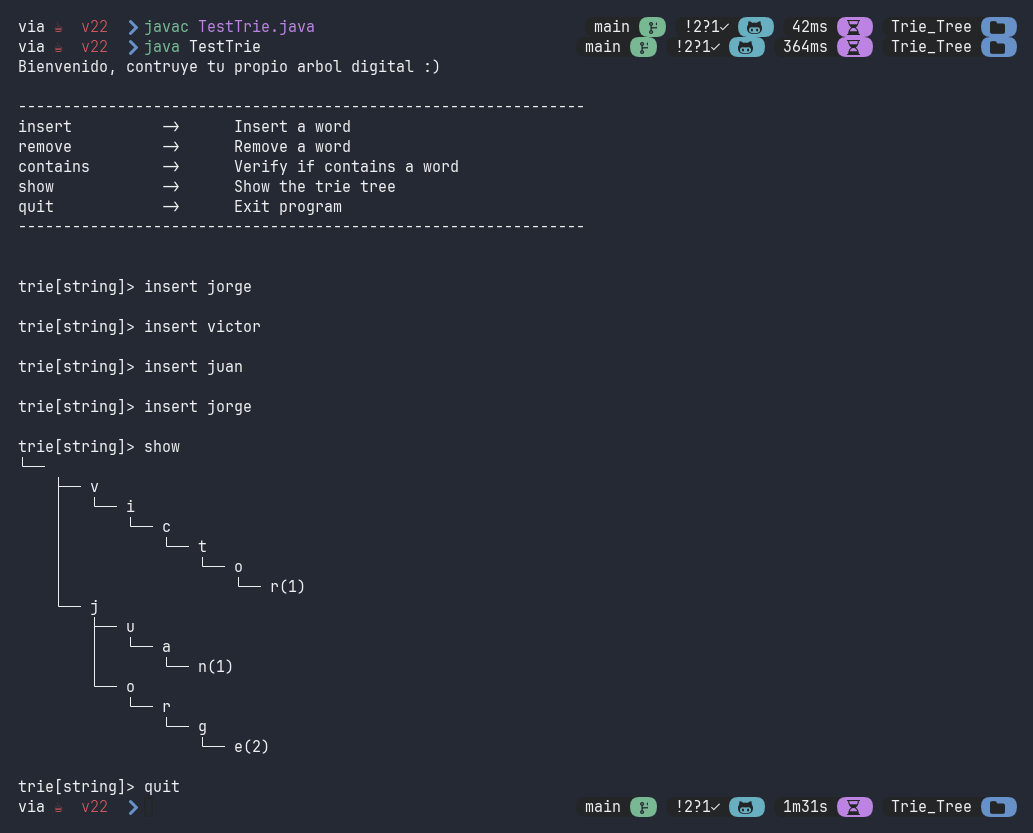
\includegraphics[width=1.0\textwidth]{img/test_trie.png}
  \caption{Trie Tree}
\end{figure}

\end{document}
